\documentclass[conference]{IEEEtran}
%\IEEEoverridecommandlockouts
% The preceding line is only needed to identify funding in the first footnote. If that is unneeded, please comment it out.
\usepackage{cite}
\usepackage[utf8]{inputenc}
\usepackage[T1]{fontenc}
% \usepackage{flushend}
\usepackage{amsmath,amssymb,amsfonts}
\usepackage{siunitx}

\usepackage{algorithm}
\usepackage{algpseudocode}
\algnewcommand{\LineComment}[1]{\Statex \(\triangleright\) #1}

\usepackage{textcomp}
\usepackage{xcolor}
\usepackage{listings}
\usepackage[hidelinks]{hyperref}
\usepackage{multirow}
\usepackage{setspace}
\usepackage{enumitem}
\usepackage[epsilon]{backnaur}
\usepackage{booktabs}

\ifCLASSOPTIONcompsoc
  \usepackage[caption=false, font=normalsize, labelfont=sf, textfont=sf]{subfig}
\else
  \usepackage[caption=false, font=footnotesize]{subfig}
\fi
\usepackage{upquote}
% nounderscore added so that this package doesn't break underscores in references.
\usepackage[nounderscore]{syntax}

% Used to suppress useless warnings when including our generated figures
\pdfsuppresswarningpagegroup=1

% Used to get around pandoc not supporting wide figures by default.
\newenvironment{widefig}{\renewenvironment{figure}{\begin{figure*}[tb]\centering}{\end{figure*}}}

\usepackage{graphicx,grffile,svg,epstopdf}
\makeatletter
\def\maxwidth{\ifdim\Gin@nat@width>\linewidth\linewidth\else\Gin@nat@width\fi}
\def\maxheight{\ifdim\Gin@nat@height>\textheight\textheight\else\Gin@nat@height\fi}
\makeatother
% Scale images if necessary, so that they will not overflow the page
% margins by default, and it is still possible to overwrite the defaults
% using explicit options in \includegraphics[width, height, ...]{}
\setkeys{Gin}{width=\maxwidth,height=\maxheight,keepaspectratio}
% Set default figure placement to htbp
\makeatletter
\def\fps@figure{tbp}
\makeatother

\providecommand{\tightlist}{%
  \setlength{\itemsep}{0pt}\setlength{\parskip}{0pt}}

\begin{document}

\title{An Approach Towards Merging Grammars}

\author{%
\IEEEauthorblockN{Isaac Griffith and Rosetta Roberts}
\IEEEauthorblockA{
  Empirical Software Engineering Laboratory\\
  Informatics and Computer Science\\
  Idaho State University\\
  Pocatello, Idaho, 83208\\
  Email: \{grifisaa@isu.edu, roberose@isu.edu\}}
  }

\maketitle

\begin{abstract}
Multilingual parsing has been found to be a difficult task which island
grammar based parsers have been demonstrated to excel at. In order to
automate the process of creating multilingual island grammar based
parsers, which has not been done, there is a need for a method of
automatically merging grammars. Such a method is presented in this
paper. This paper also evaluates the change in overall maintenance
effort and complexity of grammars caused by varying the threshold value
used to determine when similar productions can be merged. To show this,
we conducted two experiments each using a factorial design. Data for
both experiments was gathered from the ANTLR grammars-v4 repository.
Both experiments show that any merging of similar productions decreases
the maintenance effort and complexity of the resulting grammar. The
decrease was found to be more significant for lower threshold values.
This paper presents the initial steps towards the automated construction
of island and tolerant grammars for the purpose of multilingual parsing.
\end{abstract}

\begin{IEEEkeywords}
Island Grammars, Automated Grammar Formation, Software Language
Engineering
\end{IEEEkeywords}

% Decreases the vertical distance between rules in grammars from the syntax package
\setlength{\grammarparsep}{1pt}

\IEEEtriggeratref{6}

\hypertarget{sec:introduction}{%
\section{Introduction}\label{sec:introduction}}

Modern software development practice has led to an increasing number of
software systems created using multiple languages. As an example, the
modern web application is typically constructed using 5 or more
languages (e.g.~SQL, Java, TypeScript, HTML, CSS). Such multilingual
codebases present a difficult challenge to the development and
maintenance of source code analysis tools
\cite{mushtaqMultilingualSourceCode2017}. Current source analysis tools
typically address this challenge using a combination of multiple parsers
(one per supported language).

Code analysis tools have become an essential part of modern coding
\cite{kirkovSourceCodeAnalysis}. Using these tools, software engineers
find bugs, identify security flaws, increase product quality, and comply
with business rules and regulations. These tools have been integrated
into software build processes and integrated into their pipelines for
quality assurance and other services
(e.g.~SonarQube\texttrademark \footnote{\url{https://sonarqube.org}}).

Island grammars have been shown to be a solution to the problem of
developing multilingual parsers
\cite{synytskyyRobustMultilingualParsing2003}. Though useful, the
technique requires the manual combination of selected components from
source grammars, a process which can be cumbersome to maintain as these
grammars evolve. To overcome this, we propose an automated method to
reduce the initial time-consuming manual process and the further
difficulty of maintaining the constructed island grammar. In this paper
we discuss the capability to correctly combine grammar productions
together without reducing the grammar's ability to define key aspects of
interest, a key component to the automated construction of island
grammars.

The automated merging of grammars is an important and necessary step in
the evolution of island grammar research. The capability to automate
grammar merging addresses the key issues found in the initial
construction and further maintenance of island grammars. To evaluate
this hypothesis, we used the Goal-Question-Metric (GQM) paradigm
\cite{caldieraGoalQuestionMetric1994} to form the following research
goal: Evaluate an automated approach for the purpose of automating the
merging of grammar rules with respect to the maintenance effort and
complexity from the point of view of software language engineers in the
context of the creation of tolerant and island grammars. The solution
proposed will allow tool designers to develop source code analysis tools
which support multiple programming languages in an efficient and
maintainable way.

\hypertarget{organization}{%
\subsection*{Organization}\label{organization}}
\addcontentsline{toc}{subsection}{Organization}

The remainder of this paper is organized as follows.
Section~\ref{sec:background} discusses the theoretical foundations and
alternative approaches related to this work. Section~\ref{sec:approach}
details our approach to automate the merging of grammars which forms the
foundation of an initial approach to automating the creation of
multilingual parsers, which we call SIGMA.
Section~\ref{sec:experimental_design} details the design of experiments
which evaluate the proposed approach and its parameterization.
Section~\ref{sec:results} presents the results of the experiments.
Section~\ref{sec:discussion} presents a discussion of the results and
their interpretation in light of other studies.
Section~\ref{sec:threats} details the threats to the validity of this
study. Finally, this paper is concluded in
Section~\ref{sec:conclusions}.

\hypertarget{sec:background}{%
\section{Background and Related Work}\label{sec:background}}

\hypertarget{sec:foundations}{%
\subsection{Theoretical Foundations}\label{sec:foundations}}

A context free grammar, \(G\), can be described as
\(G = (V,\Sigma{},P,S)\)
\cite{haoxiangLanguagesMachinesIntroduction1988}, where \(V\) is the set
of non-terminal symbols, \(\Sigma\) is the set of terminal symbols,
\(P \subseteq V \times (V\cup\Sigma)^*\) is the set of productions
describing how the symbols of \(V\) can be substituted for other
symbols, and \(S \in V\) is the starting symbol. Each production is
written as \(a \rightarrow b\) with \(a \in V\) and
\(b \in (V\cup\Sigma)^*\). When \(b\) is the empty string, the
production is denoted by \(a \rightarrow \varepsilon\). A string, \(s\),
is called a \emph{valid sentence} for a grammar if it can be created by
repeated application of the productions of that grammar
\cite{moonenGeneratingRobustParsers2001}. \(L(G)\) denotes the set of
all valid sentences, or language, of grammar \(G\).

Island Grammars are a specialized form of context free grammar which
include the addition of a set of interests. These interests are used to
focus the grammar on the set of language components most of interest to
the grammar developers. An island grammar is formally defined as the
following tuple \(G' = (V,\Sigma{},P,S, I)\)
\cite{moonenGeneratingRobustParsers2001}, where \(I\) is the set of
interests. These interests, as noted, define the components to which the
grammar is focused, these are also known as islands. The remaining
components of a language are reduced down into one or more catchall
productions referred to as water
\cite{moonenGeneratingRobustParsers2001}. This has the effect of
reducing the complexity of the grammar. An island grammar, \(G'\),
derived from a grammar, \(G\), has a language \(L(G')\) which satisfies
the following property: \(L(G') \supset L(G)\). Island grammars offer
several advantages over regular grammars for many applications including
faster development time, lower complexity, and better error tolerance.
Due to this, island grammars have been used for many applications
including documentation extraction and processing
\cite{deursenBuildingDocumentationGenerators1999}, impact analysis
\cite{moonenLightweightImpactAnalysis2002}, and extracting code embedded
in natural language documents
\cite{bettenburgWhatMakesGood2008,bacchelliExtractingStructuredData2011}.
Of particular interest to our research is their use for creating
multilingual parsers \cite{synytskyyRobustMultilingualParsing2003},
which inspired this research, and research into the development of
tolerant grammars
\cite{klusenerDerivingTolerantGrammars2003,goloveshkinTolerantParsingSpecial2018,kursBoundedSeas2015}.

\hypertarget{sec:related}{%
\subsection{Alternative Approaches}\label{sec:related}}

Using an intermediate representation (IR), such as
Java\texttrademark~bytecode or Microsoft IL, is a common method for
performing operations on multilingual code bases. This allows code
analysis tools to be built around the language(s) defined by the IR
rather than having to deal with each of the different languages
individually. However, using an IR doesn't work when analyzing systems
created from languages that do not share a common IR
\cite{linosMetricsToolMultilanguage}. Using an IR also doesn't work if
performing manipulations of source code or if there isn't a clear
correspondence between a source language and its IR. An example of this
can be seen for PIT \cite{colesPITPracticalMutation2016}, a Java
mutation testing framework. Even though their system is designed around
transforming and manipulating Java bytecode, the system struggles with
handling bytecode generated by other JVM languages. However, they still
have had limited success with other JVM languages
\cite{clarkeExperimentingMutationTesting2016}.

Another approach that's been developed for analyzing multilingual
systems is through the use of a separate parser for each language.
Constructing and integrating each parser for each language can be both
difficult and time consuming, and thus it is better to use existing
parsers \cite{janesHowCalculateSoftware2013}. Using existing parsers,
one can modify the abstract syntax trees into a language independent
form. The problem one contends with in this approach is these parsers
may be written in a variety of languages. The use of an existing Island
Grammar \cite{synytskyyRobustMultilingualParsing2003} may alleviate
these issues, but typically they tend to be specific to their particular
problem and their construction is currently a time-consuming manual
process.

\hypertarget{sec:approach}{%
\section{Approach}\label{sec:approach}}

In order to generate an island grammar from one or more source grammars,
there is a need to merge components of the source grammar(s) to reduce
or deduplicate the final grammar. Such a technique can be used to reduce
the island components. Thus, the focus of this paper is the development
of a technique to merge grammars together, and is depicted in
Fig.~\ref{fig:approach}. The process is as follows:

\begin{enumerate}
\def\labelenumi{\arabic{enumi}.}
\tightlist
\item
  Parse the input grammars.
\item
  Trivially merge the grammars into a single grammar.
\item
  Normalize the merged grammar.
\item
  Calculate the similarity between each pair of rules.
\item
  Merge the two most similar rules.
\item
  Repeat steps 4 and 5 until the two most similar rules are no longer
  similar.
\item
  Final Normalization of Merged Grammar
\item
  Output the merged grammar.
\end{enumerate}

\begin{figure}
\hypertarget{fig:approach}{%
\centering
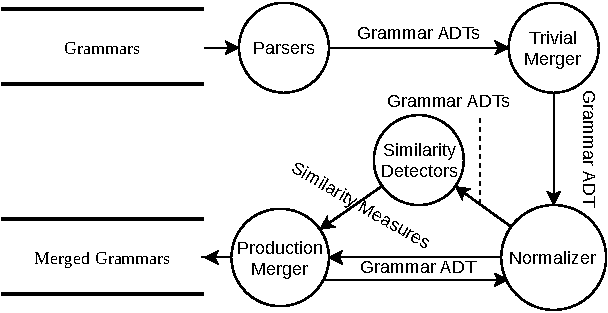
\includegraphics{images/paper/SIGMA-DFD.pdf}
\caption{Data flow diagram of merging process.}\label{fig:approach}
}
\end{figure}

The remainder of this section presents the details of each of these
steps and utilizes a running example based on the the two grammars
depicted in Fig.~\ref{fig:grammar_g1} and Fig.~\ref{fig:grammar_g2}.

\begin{figure}[tb]
 \centering
 \subfloat[Grammar $G_1$.]{
   \label{fig:grammar_g1}
   \begin{minipage}[t]{0.2\textwidth}

\begin{grammar}
<S> ::= <A> | <B>

<Y> ::= <A> | `y'

<A> ::= `a' $\varepsilon$ <B> <C>

<C> ::= `c'

<B> ::= `b' `d'

\end{grammar}

 \end{minipage}
 }
 \qquad
 \subfloat[Grammar $G_2$.]{
   \label{fig:grammar_g2}
   \begin{minipage}[t]{0.2\textwidth}

\begin{grammar}
<S> ::= <C> | <D>

<Z> ::= <S> | `z'

<C> ::= `c'

<D> ::= `a' `d' (`e' | `c') | (<C> | `b')

\end{grammar}

 \end{minipage}
 }
 \caption{Example grammars used to demonstrate merging procedure.}
\end{figure}

\hypertarget{sec:parsing}{%
\subsection{Parsing}\label{sec:parsing}}

\begin{figure}
\hypertarget{fig:grammar_class_diagram}{%
\centering
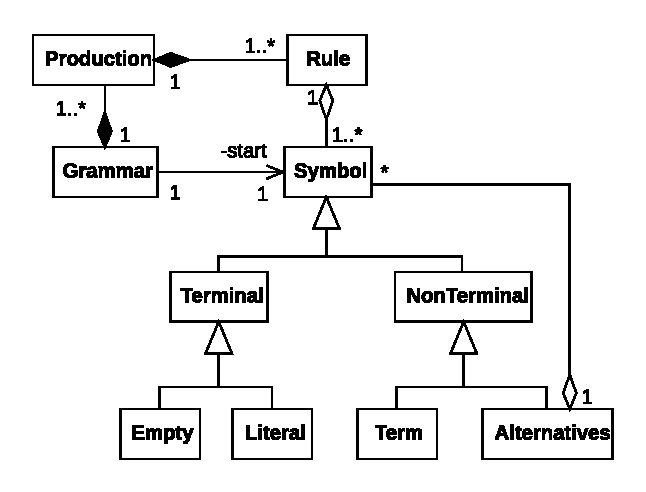
\includegraphics{images/paper/diagram.eps}
\caption{Class diagram of internal domain model used to represent
grammars throughout the merging
process.}\label{fig:grammar_class_diagram}
}
\end{figure}

The initial step of the process is the translation of the textual
representations of the grammars into an instance of our domain model,
depicted in Fig.~\ref{fig:grammar_class_diagram}. In our experiments we
analyzed grammars stored in the ANTLR 4 grammar format. Thus, to create
instances of our model, we processed the grammars using an ANTLR 4
grammar parser. This parser constructs an abstract syntax tree which is
then converted into an instance of the domain model.

The conversion process is complicated by the fact that the ANTLR 4
representation is not fully compatible with our BNF based domain model.
To resolve this, we removed or converted all non-BNF features except for
\emph{dot}, \emph{character range}, \emph{character class}, and
\emph{not} rules. These operators act as they do in any typical regular
expression language. The \emph{dot}, \emph{character range}, and
\emph{character class} operators, were converted to special terminal
symbols. \emph{Not} rules were retained by extracting each into its own
rule. For example:

\begin{verbatim}
        A: 'a' . ~('b' | 'c')
\end{verbatim}

\noindent would be converted to:

\begin{grammar}
      <A> ::= `a' DOT <Generated-1>

      <Generated-1> ::= \textasciitilde<Generated-2>

      <Generated-2> ::= `b' | `c'

\end{grammar}

\noindent The \emph{not} rules are ignored completely by this process
except for when detecting and merging duplicate rules.

\hypertarget{sec:trivial_merge}{%
\subsection{Trivial Merge}\label{sec:trivial_merge}}

The initial merge is the combination of the start productions of the
grammars to be combined. First, a new start symbol is created in the new
grammar. Productions are also added from this symbol to each of the
source grammars' start productions. The trivial merging of grammars
\(G_1\) and \(G_2\) yields the grammar \(G_3\) depicted in
Fig.~\ref{fig:grammar_g3}. Where the original source grammar start
productions are renamed S1 and S2 representing the start productions for
both \(G_1\) and \(G_2\), respectively.

\begin{figure}[tb]
 \centering
  \begin{minipage}[t]{.2\textwidth}

\begin{grammar}
<S> ::= <\(S_1\)> | <\(S_2\)>

<$S_1$> ::= <A> | <B>

<Y> ::= <A> | `y'

<A> ::= `a' $\varepsilon$ <B> <\(C_1\)>

<$C_1$> ::= `c'

<B> ::= `b' `d'

<$S_  2$> ::= <\(C_2\)> | <D>

<Z> ::= <S> | `z'

<$C_2$> ::= `c'

<D> ::= `a' `d' (`e' | `c') | (<\(C_2\)> | `b')

\end{grammar}

  \end{minipage}
 \caption{Grammar $G_3$. The result of trivially merging $G_1$ and $G_2$.}\label{fig:grammar_g3}
\end{figure}

\hypertarget{sec:normalization}{%
\subsection{Normalization}\label{sec:normalization}}

Next, the trivially merged grammar is normalized. The normalization
process works to eliminate unused rules, simplify productions, merge
equivalent rules, eliminate unit rules, expand productions, and collapse
compatible productions. We leave the details of this process to another
paper because the complexity of this process can't be fully explained in
this paper without detracting from this paper's focus on the merging of
similar rules.

\hypertarget{sec:similarity}{%
\subsection{Measuring Rule Similarity}\label{sec:similarity}}

The fourth step of this approach measures the similarity between each
pair of productions. This measure is used by the fifth step to identify
merge candidate pairs. In this section, describe the two similarity
metrics corresponding to the two forms (defined in
Section~\ref{sec:normalization}) of productions produced by the
normalization process. We note productions of different forms will have
a similarity of 0.

\hypertarget{term-similarity}{%
\subsubsection{Term Similarity}\label{term-similarity}}

The first similarity metric measures the similarity between two
productions of form 1. As an example, assume we have the following two
productions:

\begin{grammar}
<$P_a$> ::= `a' <A> `b' `c'

<$P_b$> ::= <A> <B> `b' `a'

\end{grammar}

The first step towards measuring the similarity between these
productions is aligning the productions using the Longest Common
Subsequence (LCS) algorithm \cite{cormenIntroductionAlgorithms2001}.

\begin{verbatim}
'a' <A>     'b'     'c'
    <A> <B> 'b' 'a'
\end{verbatim}

Once aligned, the number of aligned terms is divided by the total number
of terms, as described in (\ref{eqn:metric1}):

\begin{eqnarray}\label{eqn:metric1}
S_1 & = & \frac{2|\textsc{LCS}(P_a, P_b)|}{|P_a| + |P_b|}.
\end{eqnarray}

\noindent Applying (\ref{eqn:metric1}) to the example,
\texttt{\textless{}A\textgreater{}} and
\texttt{\textquotesingle{}b\textquotesingle{}} are each counted twice
because they occur in both sequences of terms. The total number of terms
across both productions is 8. The total similarity score is computed as,
\(S_1 = \frac{4}{8} = .5\).

\hypertarget{alternatives-similarity}{%
\subsubsection{Alternatives Similarity}\label{alternatives-similarity}}

The second similarity metric measures the similarity between two
productions of form 2. As an example, assume we have the following two
productions:

\begin{grammar}
<\(P_a\)> ::= `a' | <A> | `b' | `c'

<\(P_b\)> ::= <A> | <B> | `b' | `a'

\end{grammar}

Similar to the previous metric, this metric calculates the number of
common alternatives divided by the total number of alternatives.
However, because the order of the alternatives does not matter, a
different approach to measure the common alternatives is applied. In
this approach an alternative is counted as common to both if it occurs
in both productions. Equation (\ref{eqn:metric2}) describes how to
calculate the similarity score using this method:

\begin{eqnarray}\label{eqn:metric2}
S_2 & = & \frac{2|P_a \cap P_b|}{|P_a| + |P_b|}.
\end{eqnarray}

\noindent Applying (\ref{eqn:metric2}) to the example, the common
elements are \texttt{\textless{}A\textgreater{}},
\texttt{\textquotesingle{}a\textquotesingle{}}, and
\texttt{\textquotesingle{}b\textquotesingle{}}. The similarity score is
computed as \(\frac{2\cdot 3}{8} = 0.75.\)

\hypertarget{sec:merging_similar}{%
\subsection{Merging Similar Rules}\label{sec:merging_similar}}

Once the two most similar productions are detected they are then merged
together. Similar to the process of measuring similarity, there are two
form specific processes for merging similar productions. This process
relies upon a minimal similarity threshold, \(M_s\), above which similar
productions are merged.

\hypertarget{merging-similar-terms}{%
\subsubsection{Merging Similar Terms}\label{merging-similar-terms}}

To merge two productions of the first form, the LCS alignment produced
while measuring the similarity between terms is used. Initially, each
pair of subsequences that do not align are identified. In the previous
example, the identified unaligned pairs of subsequences are:
(\texttt{\textquotesingle{}a\textquotesingle{}}, \(\varepsilon\)),
(\(\varepsilon\), \texttt{\textless{}B\textgreater{}}), and
(\texttt{\textquotesingle{}a\textquotesingle{}},
\texttt{\textquotesingle{}c\textquotesingle{}}). Each pair of unaligned
subsequence is then substiuted with the union of the two subsequences.
As an example, the prior example sequences of terms would merge to:
\(\left<P_{a+b}\right>\) ::=
(\texttt{\textquotesingle{}a\textquotesingle{}} \textbar{}
\(\varepsilon\)) \(\left<A\right>\) (\(\varepsilon\) \textbar{}
\(\left<B\right>\)) \texttt{\textquotesingle{}b\textquotesingle{}}
(\texttt{\textquotesingle{}c\textquotesingle{}} \textbar{}
\texttt{\textquotesingle{}a\textquotesingle{}}).

\hypertarget{merging-similar-alternatives}{%
\subsubsection{Merging Similar
Alternatives}\label{merging-similar-alternatives}}

Merging two productions of the second form is simpler than the first
form. The merged production produced simply contains all alternatives
that are in either constituent production. As an example, the prior
example productions \(\left<P_a\right>\) and \(\left<P_b\right>\) would
be merged to the following: \(\left<P_{a+b}\right>\) ::=
\texttt{\textquotesingle{}a\textquotesingle{}} \textbar{}
\(\left<A\right>\) \textbar{} \(\left<B\right>\) \textbar{}
\texttt{\textquotesingle{}b\textquotesingle{}} \textbar{}
\texttt{\textquotesingle{}c\textquotesingle{}}.

\hypertarget{sec:grammar_output}{%
\subsection{Grammar Output}\label{sec:grammar_output}}

At the end of this process, we output the merged and transformed
grammar. The output is generated by simply visiting every production in
the grammar. As each production is visited a corresponding ANTLR 4
production is generated and written out.

\hypertarget{sec:experimental_design}{%
\section{Experimental Design}\label{sec:experimental_design}}

This section describes the overall experimental design used to evaluate
the grammar merging approach presented within this paper. The following
subsections detail the separate aspects of our experimental design.

\hypertarget{sec:exp_goals}{%
\subsection{Goals, Hypotheses, and Variables}\label{sec:exp_goals}}

This subsection describes the refinement of our initial research goal,
defined in Section~\ref{sec:introduction}, into a set of actionable
research questions and metrics. Based on this set of research questions
we also identified the variables used in statistical models driving our
analytical procedures. We begin with the research questions and metrics.

Following the GQM paradigm, research goal RG can be decomposed into the
following set of research questions:

\begin{enumerate}[label={\textbf{RQ\arabic*}},left=.2in]

\item What is the effect that this process has on the maintenance effort between the source grammars and the grammar produced by this approach?

 \textbf{Rationale:} \textit{It is expected that the merging of grammar components will reduce the maintenance effort required.}

 \item What is the effect that this process has on the complexity between the source grammars and the grammar produced by this approach?

 \textbf{Rationale:} \textit{It is expected that the merging and reduction of grammar components will reduce the complexity of the grammar, thus making the grammar easier to understand and read.}

\end{enumerate}

\noindent In addition to these research questions we have selected the
following metrics to assess the results of the approach used:

\begin{enumerate}[label={\textbf{M\arabic*}},left=.2in]

\item Effort -- To assess the effort required to maintain a grammar, we utilize the Halstead Effort measure for grammars as defined by Power and Malloy \cite{powerMetricsSuiteGrammarbased2004}.
  \item Complexity -- To assess the complexity of a grammar, we utilize McCabe's Cyclomatic Complexity metric for grammars defined by Power and Malloy \cite{powerMetricsSuiteGrammarbased2004}.

\end{enumerate}

The dependent variables in the experiments, as indicated by the above
research questions, are maintenance effort and complexity. Specifically,
we are concerned with the change between the trivial merge state and the
final grammar in terms of the effort and complexity of the grammar.
Thus, the dependent variables of concern are:

\begin{itemize}
\tightlist
\item
  \(\Delta HAL\) -- the change in Halstead Effort as measured after the
  normalization phase prior to the final merge phase, and after the
  final merge phase and before generating the output grammar.
\item
  \(\Delta MCC\) -- the change in complexity as measured after the
  normalization phase prior to the final merge phase, and after the
  final merge phase and before generating the output grammar.
\end{itemize}

\noindent The independent variables we are concerned with are:

\begin{itemize}
\tightlist
\item
  Similarity Threshold -- the parameter guiding the similarity
  measurements used in the merging process. The values used in the
  experiments are 0.001, 0.25, 0.5, 0.75, and 1.0.
\item
  Size -- the size of the grammar as defined by measuring its number of
  productions (PROD) \cite{powerMetricsSuiteGrammarbased2004}, and
  threshold this value into three distinct categories: Small, Medium,
  and Large, as defined in Section~\ref{sec:subjects}.
\end{itemize}

\hypertarget{sec:design}{%
\subsection{Design}\label{sec:design}}

To evaluate the approach we elected to conduct two experiments. The
first experiment evaluates the effect the approach has on the
maintenance effort necessary to maintain a merged grammar as compared to
its combined source grammars. The second experiment evaluates the effect
the approach has on the complexity of the merged grammar as compared to
its combined source grammars. These experiments utilize a Factorial
Design, with a single dependent variable (\(\Delta HAL\),
\(\Delta MCC\)), a treatment factor \(Similarity Threshold\) and the
grouping factor \(Size\).

\hypertarget{sec:subjects}{%
\subsection{Experimental Units}\label{sec:subjects}}

\begin{table*}[tb]
\centering
\caption{Grammars randomly selected from each size category used in the experiments.}
\label{tbl:grammar_metrics}
\begin{tabular}{|c|l|}
\hline
Category & Grammars\tabularnewline
\hline
\hline
\multirow{2}{*}{S} & brainfuck, cmake, csv, inf, lcc, pdn,\tabularnewline
\cline{2-2}
 & properties, quakemap, sexpression, tsv, url, useragent\tabularnewline
\hline
\multirow{2}{*}{M} & cto, dart2, flatbuffers, fusion-tables, lua, pascal\tabularnewline
\cline{2-2}
 & python2, romannumerals, sgf, stacktrace, webidl, z-ops\tabularnewline
\hline
\multirow{2}{*}{L} & cql3, edif300, fortran77, idl, informix, java9\tabularnewline
\cline{2-2}
 & kotlin, objc-two-step, powerbuilder, rexx, sharc, swift2\tabularnewline
\hline
\end{tabular}
\end{table*}

In these experiments, the experimental units are pairs of grammars
selected from the ANTLR 4 \cite{parrDefinitiveANTLRReference2012}
grammar repository\footnote{\url{https://github.com/antlr/grammars-v4}}.
The sys-verilog grammar was excluded because of errors while parsing it.
At the time of this writing, the repository contained 198 individual
grammars from a variety of general purpose and domain specific
languages.

The process used to select the grammar pairs for each experiment is
depicted in Fig.~\ref{fig:selection_process} and works as follows.
Initially, for each of the grammars in the repository we collected a
combination of metadata and metric measurements. The metadata consists
of the language represented by the grammar, the version of that language
(if applicable) and the following metrics (selected from the metrics
suite by Power and Malloy \cite{powerMetricsSuiteGrammarbased2004}):

\begin{itemize}
\tightlist
\item
  TERM -- the number of terminals.
\item
  VAR -- the number of defined non-terminals.
\item
  PROD -- the number of productions.
\item
  MCC -- McCabe's cyclomatic complexity.
\end{itemize}

\begin{figure}
\hypertarget{fig:selection_process}{%
\centering
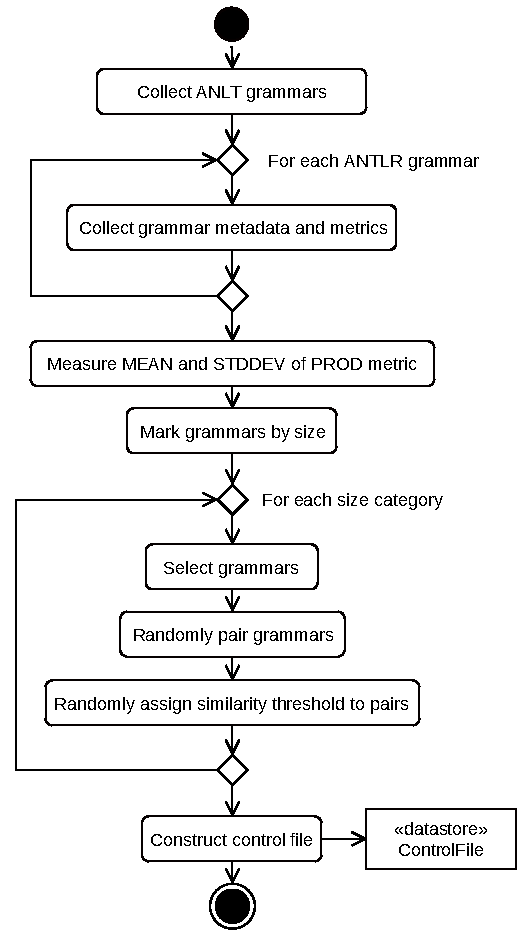
\includegraphics{images/paper/select_process_1.pdf}
\caption{Activity diagram describing how control files representing each
replication are created.}\label{fig:selection_process}
}
\end{figure}

Using the resulting measures of these metrics, the grammar dataset was
subdivided into three categories (Small, Medium and Large) based on the
logarithm of PROD (as the values were log-normal distributed). This
subdivision was based on statistically construction thresholds, as per
Lanza and Marinescu \cite{lanzaObjectorientedMetricsPractice2011}.
Category threshold values are defined as: Small-Medium:
\(10^{\mu_{PROD} - \sigma_{PROD}} = 10^{1.8404 - 0.5371} = 20.1084\) and
Medium-High:
\(10^{\mu_{PROD} + \sigma_{PROD}} = 10^{1.8404 + 0.5371} = 238.4995\).
Using these thresholds each grammar is then grouped into one of the
three categories.

Using these categories as the grouping factor in the experiments, we can
then begin the sampling process. As we have selected a \(3\times 5\)
factorial design, each replication of each of the two experiments
requires 15 grammar pairs (5 per size category). Based on our
replication analysis (described in Section~\ref{sec:analysis_proc}) we
have identified a need for a total of 5 replications. Thus, for each
size category we require a total of 50 grammar pairs per experiment
yielding a need for 100 total grammar pairs. To meet this requirement we
randomly select (without replication) 12 grammars, per size category.
From these 12 grammars there are \(12 \choose 2\) = 66 combinations
without replication of which we randomly select 5 pairs per replication
per experiment. The grammars selected and their pairings per
experiment/replication are depicted in Table~\ref{tbl:grammar_metrics}.

Once the grammar pairs are selected, they are assigned a treatment value
for use during the experiment execution and data collection phase. For
each size category per replication per experiment, the set of five
grammar-pairs are assigned, at random, a level of the similarity
threshold treatment. The possible levels that can be assigned are 0.001,
0.25, 0.5, 0.75, and 1.0 where 1.0 is the control level.

Finally, the data generated as part of the selection process is used to
construct an experiment control file. This file is used to direct the
experimental execution system and to ensure the validity of the process.
Each control file is simply an ordered set of triples where each triple
consists of the following information:

\begin{itemize}
\tightlist
\item
  Grammar Pair - the pair of grammars to be merged together, as selected
  during the selection phase.
\item
  Treatment - the similarity threshold value assigned to the grammar
  pair during the selection phase.
\item
  Size - value of the size category, for use in constructing the data
  table.
\end{itemize}

\noindent Each replication has a separate control file to control its
execution. Thus, for each replication, the control file triples are
created and put into a list which is then randomized. This randomized
list is then output to a file which is later read in by the experimental
execution system.

\hypertarget{sec:data_coll_proc}{%
\subsection{Data Collection Procedures}\label{sec:data_coll_proc}}

\begin{figure}
\hypertarget{fig:dc_proc}{%
\centering
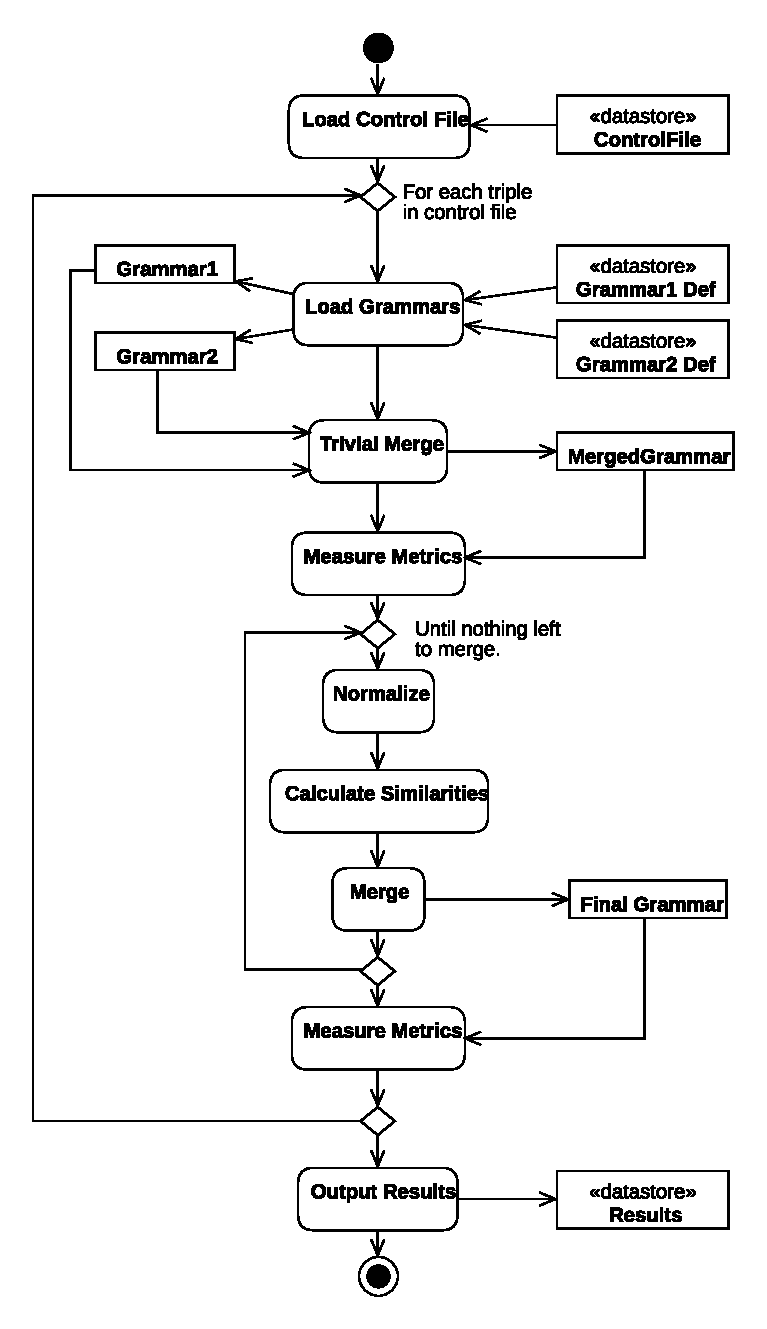
\includegraphics{images/paper/data_collect.eps}
\caption{Activity diagram showing locations in the merging process where
metrics are gathered.}\label{fig:dc_proc}
}
\end{figure}

Data collection is performed via the experiment execution system
specifically developed for this study. This system is controlled via the
control files created during the experimental unit selection process.
The data collection process follows the activity diagram depicted in
Fig.~\ref{fig:dc_proc}.

Initially, the control file is read into the system. Then, for each of
the triples in the list, the following occurs: 1.) The selected
similarity threshold value is applied. 2.) The grammars located, read
in, and trivially merged together. 3.) The combined grammar's effort or
complexity is then measured and recorded. 4.) The final merging process
is applied resulting in the final grammar. 5.) The resulting grammar's
effort or complexity is then measured and recorded.

Once all experimental units have been processed the results are exported
to a data table. This process is repeated for each replication of each
experiment. The results from each replication of each experiment are
then combined into a single data table. The combined data table is then
used during the analysis phase.

\hypertarget{sec:analysis_proc}{%
\subsection{Analysis Procedures}\label{sec:analysis_proc}}

As described in Section~\ref{sec:experimental_design}, both experiments
utilize a Factorial design
\cite{montgomeryDesignAnalysisExperiments2013}. Typically, a factorial
design experiment will utilize ANOVA to determine if there is a
difference between the effects of the factors. In this case, the
statistical model used is as follows:

\[y_{ijk} = \mu + st_i + size_j + (st * size)_{ij} \epsilon_{ijk}\]

\noindent Where:

\begin{itemize}
\tightlist
\item
  \(y_{ijk}\) is the kth value of the observation (either \(\Delta MCC\)
  or \(\Delta HAL\)) associated with the ith similarity threshold level
  and jth size level.
\item
  \(\mu\) is the baseline mean
\item
  \(st_{i}\) is the ith level of similarity threshold effect.
\item
  \(size_{j}\) is the jth level of size effect.
\item
  \((st * size)\_{ij}\) is the similarity threshold * size interaction
  effect.
\item
  \(\epsilon_{ijk}\) is the random error of the kth observation from the
  (i, j)th cell.
\end{itemize}

\noindent The hypotheses to be tested in this case are as follows:

\begin{itemize}
\tightlist
\item
  \(H_{1,0}\) : The effect of the levels of the interaction term are
  equal.
\item
  \(H_{1,A}\) : There is at least one difference between interaction
  level effects.
\item
  \(H_{2,0}\) : The effects of the levels of similarity threshold are
  equal.
\item
  \(H_{2,A}\) : There is at least one difference between similarity
  threshold level effects.
\item
  \(H_{3,0}\) : The effects of the levels of size are equal.
\item
  \(H_{3,A}\) : There is at least one difference between size level
  effects.
\end{itemize}

ANOVA has several assumptions that must first be verified. First, is the
assumption of homogeneity of variance. To evaluate this assumption, we
will use Levene's Test \cite{leveneRobustTestsEquality1960}. The next
assumption is that both the factors and errors are normally distributed.
To verify this assumption, we will use the Anderson-Darling Test for
Goodness of Fit \cite{andersonTestGoodnessFit1954} to the normal
distribution for both the errors and factor effects. Finally, there is
the assumption of independence of the observations, which is valid due
to the nature of the process.

In the case of any violations of these assumptions we will attempt to
correct the violation using a Box Cox transformation. In the case that
the assumptions are violated beyond the capability to correct, we will
be forced to utilize a non-parametric approach. Specifically, we will
use a permutation F-test
\cite{higginsIntroductionModernNonparametric2004}, in place of ANOVA.
The permutation F-test also has a set of assumptions that must be met
prior to use. The model for the permutation F-test is the same as that
of ANOVA.

In either case, the next step is to conduct the hypothesis test and make
a decision. In this case we have selected an \(\alpha\) threshold of
0.95. In the case that we reject \(H_{1,0}\) we will then conduct a
multiple-comparison procedure to compare the individual effects of each
level of the similarity threshold factor. In these experiments the
similarity threshold level of 1.0 to be the control (as noted in
Section~\ref{sec:design}). Dunnett's
\cite{dunnettMultipleComparisonProcedure1955} multiple comparison
procedure will be selected if ANOVA is used, and Steel's
\cite{steelMultipleComparisonSign1959} multiple comparison procedure (a
non-parametric technique analogous to Dunnett's) if using the
permutation F-test. Both of these comparison procedures control the
error for multiple comparisons and allow the ability to compare against
a control. In the case of Dunnett's Test we will be evaluating the
following hypotheses:

\begin{itemize}
\tightlist
\item
  \(H_{4,0}\) : There is no difference between the mean effects of
  similarity threshold effects and control effect.
\item
  \(H_{4,A}\) : There is a difference between at least one similarity
  threshold level and control.
\end{itemize}

\noindent In the case of Steel's Test we will be evaluating the
following hypotheses:

\begin{itemize}
\tightlist
\item
  \(H_{4,0}\) : There is no difference between the median effects of
  similarity threshold effects and control effect.
\item
  \(H_{4,A}\) : There is a difference between at least one similarity
  threshold level and control.
\end{itemize}

\noindent For either of these tests we will use an \(\alpha\) threshold
of 0.95.

Additionally, we are interested if there is a strict order of the effect
on \(\Delta HAL\) or \(\Delta MCC\) for the levels of the similarity
threshold factor. To evaluate this we have selected to utilize the
Jonhckheer's trend test. This is a non-parametric test to determine if
there is an \emph{a priori} ordering within independent samples
\cite{jonckheereDistributionFreeKSampleTest1954}. The hypotheses to be
tested are as follows:

\begin{itemize}
\tightlist
\item
  \(H_{5,0}\) : There is no difference in median effects of the
  similarity threshold levels.
\item
  \(H_{5,A}\) : There is a increasing trend in the effects of the
  similarity threshold levels, with at least one being a strict
  inequality.
\end{itemize}

Finally, we will also conduct a sample size analysis to determine the
number of repetitions necessary to achieve the power level necessary for
the experiments.

\hypertarget{sec:results}{%
\section{Results}\label{sec:results}}

\hypertarget{sec:desc_stats}{%
\subsection{Descriptive Statistics}\label{sec:desc_stats}}

This subsection describes the data collected via a series of descriptive
statistics. Table~\ref{tbl:descriptive} shows the mean values of
\(\Delta HAL\) and \(\Delta MCC\) for each value of the size category in
the respective experiments. Along with this table the dispersion of the
both \(\Delta HAL\) and \(\Delta MCC\) across size and similarity
threshold values is displayed in Fig.~\ref{fig:hal_box} and
Fig.~\ref{fig:mcc_box}, respectively.

\begin{table}[tb]
\caption{Descriptive Statistics.}
\label{tbl:descriptive}
\begin{tabular}{lrr}
\hline
\textbf{Size Category} & \textbf{Mean $\Delta HAL$} & \textbf{Mean $\Delta MCC$}\tabularnewline
\hline
Small & 1290.2 & 32.32\tabularnewline
Medium & 18573 & 112.7\tabularnewline
Large & 149854 & 842.4\tabularnewline
\hline
\end{tabular}
\end{table}

\begin{figure}
\hypertarget{fig:hal_box}{%
\centering
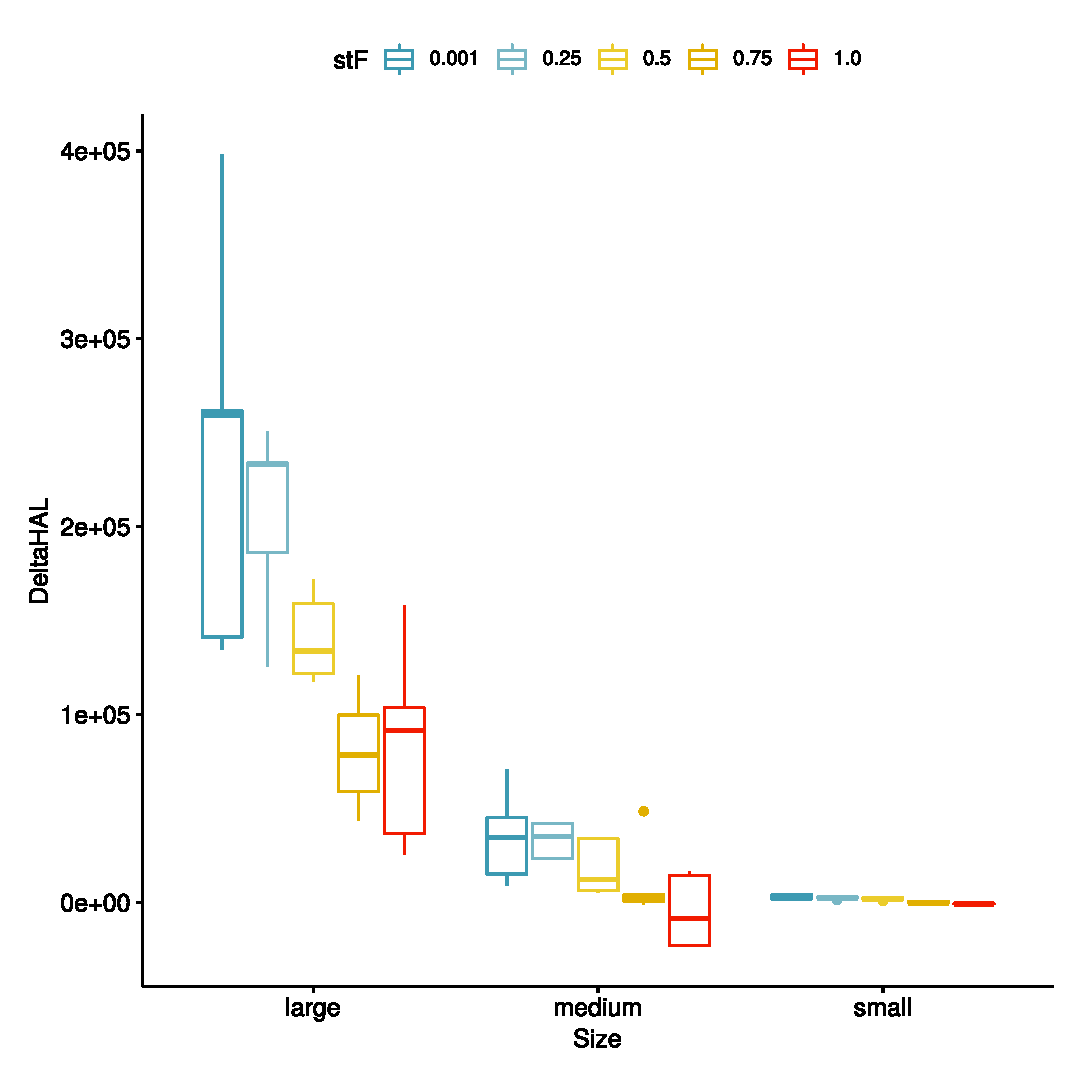
\includegraphics{images/paper/results/hal_box.eps}
\caption{Results of running the Delta HAL experiment in the form of
boxplots.}\label{fig:hal_box}
}
\end{figure}

\begin{figure}
\hypertarget{fig:mcc_box}{%
\centering
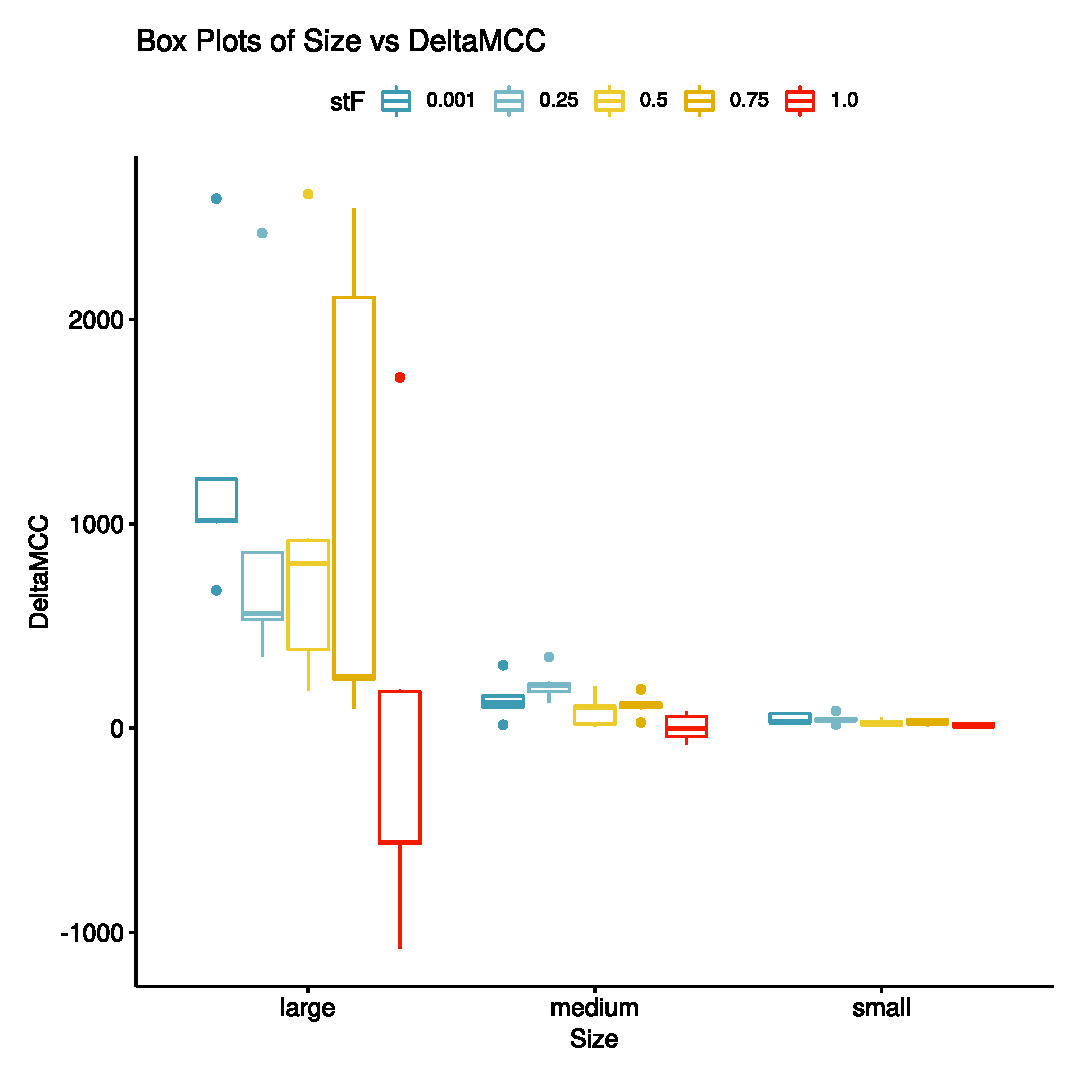
\includegraphics{images/paper/results/mcc_box.eps}
\caption{Results of running the Delta MCC experiment in the form of
boxplots.}\label{fig:mcc_box}
}
\end{figure}

\begin{figure}
\hypertarget{fig:ex1_qqplots}{%
\centering
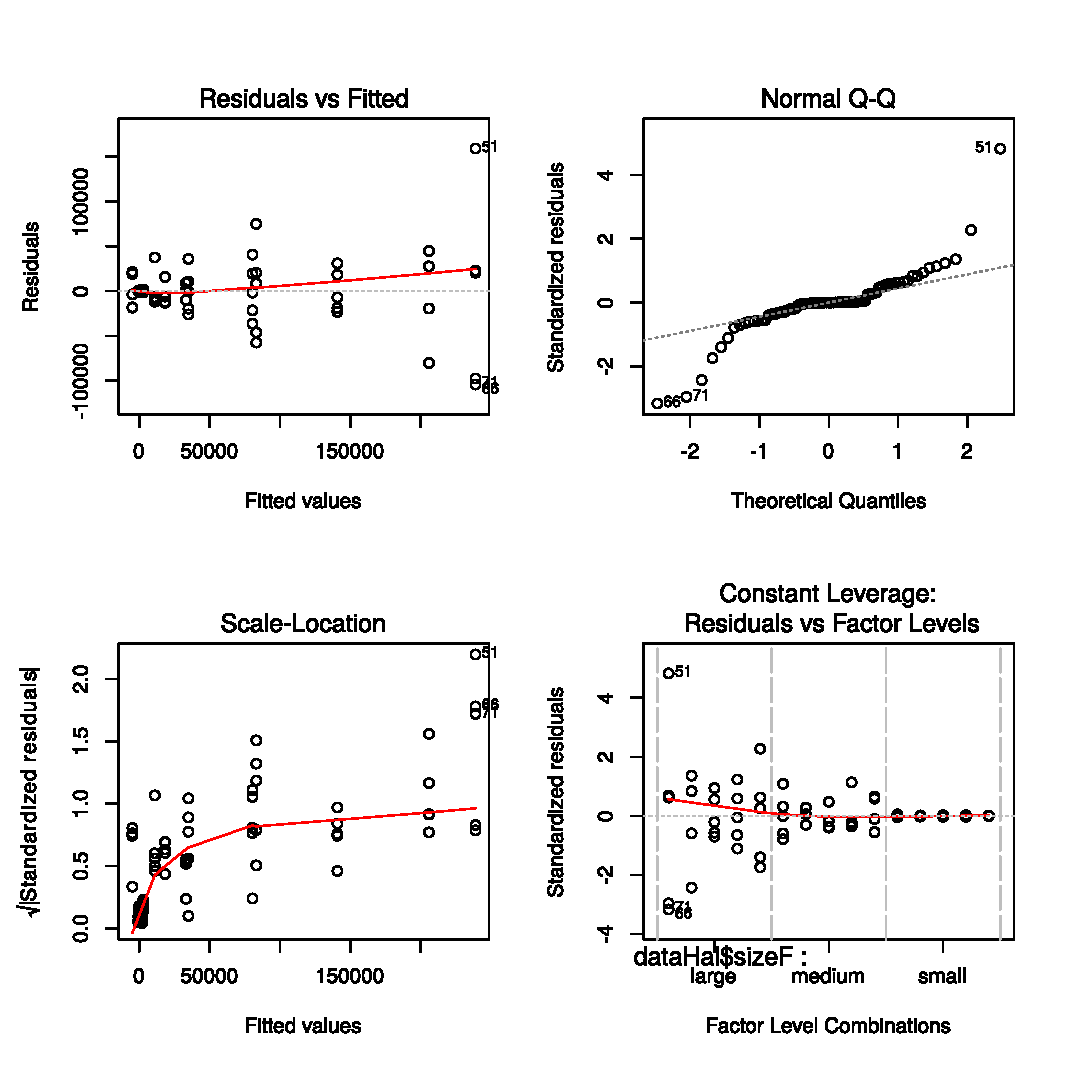
\includegraphics{images/paper/results/ex1_qqplots.eps}
\caption{Delta Hal experiment Q-Q plots.}\label{fig:ex1_qqplots}
}
\end{figure}

As we can see from the Residuals vs.~Fitted plot, depicted in
Fig.~\ref{fig:ex1_qqplots}, the homogeneity of variance assumption is
not met. To validate this observation we used Levene's Test. In this
test, the null-hypotheses (\(H_0\)) asserts that the variance is equally
distributed. As expected, from our observations of the Residuals vs
Fitted Values plot, the test produced an F-value of 19.962 and a p-value
of 1.267e-07 indicating that we should reject the null hypothesis that
there is a homogeneity of variance.

The Normal Q-Q plot, depicted in Fig.~\ref{fig:ex1_qqplots}, indicates
that the normality of the residuals assumption is also violated. To
validate this observation we conducted both an Anderson-Darling GOF test
against the Normal distribution. In this test the null-hypothesis
(\(H_0\)) is that the empirical distribution is Normal. The results show
that the A statistic has a value of 6.8257 and an associated p-value of
\textless{} 2.2e-16 which indicates that we can reject the
null-hypothesis. These results confirm our initial observation that the
results are not normally distributed.

\begin{figure}
\hypertarget{fig:ex1_interaction}{%
\centering
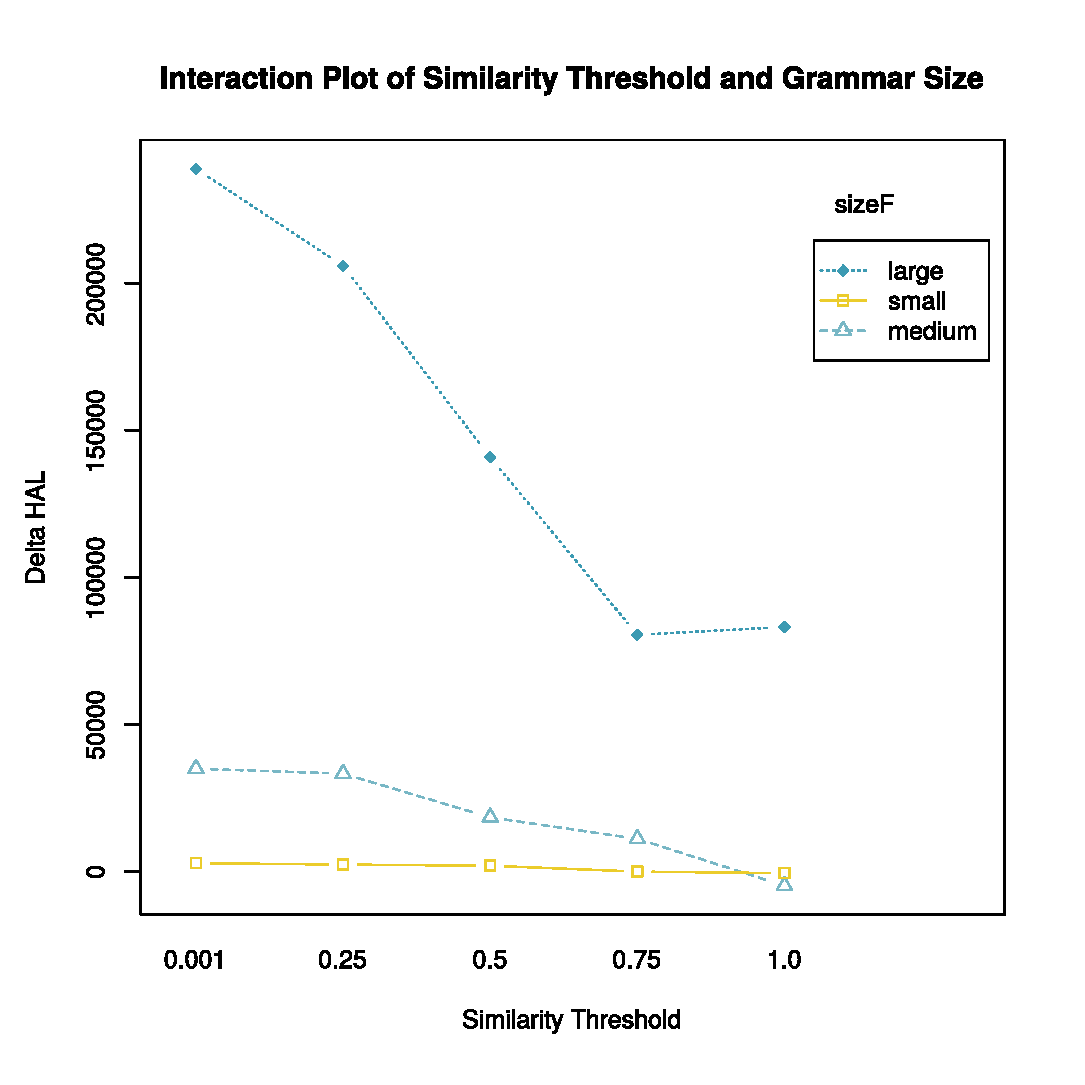
\includegraphics{images/paper/results/ex1_interaction.eps}
\caption{Delta HAL experiment interaction
plot.}\label{fig:ex1_interaction}
}
\end{figure}

The interaction plot, depicted in Fig.~\ref{fig:ex1_interaction},
indicates that there is an interaction between the small and medium
levels as the similarity threshold changes from 0.75 to 1.0. This
indicates that the assumption that the block and treatment do not
interact and that an RCBD design is inappropriate and a factorial design
would be more accurate.

\begin{figure}
\hypertarget{fig:ex2_qqplots}{%
\centering
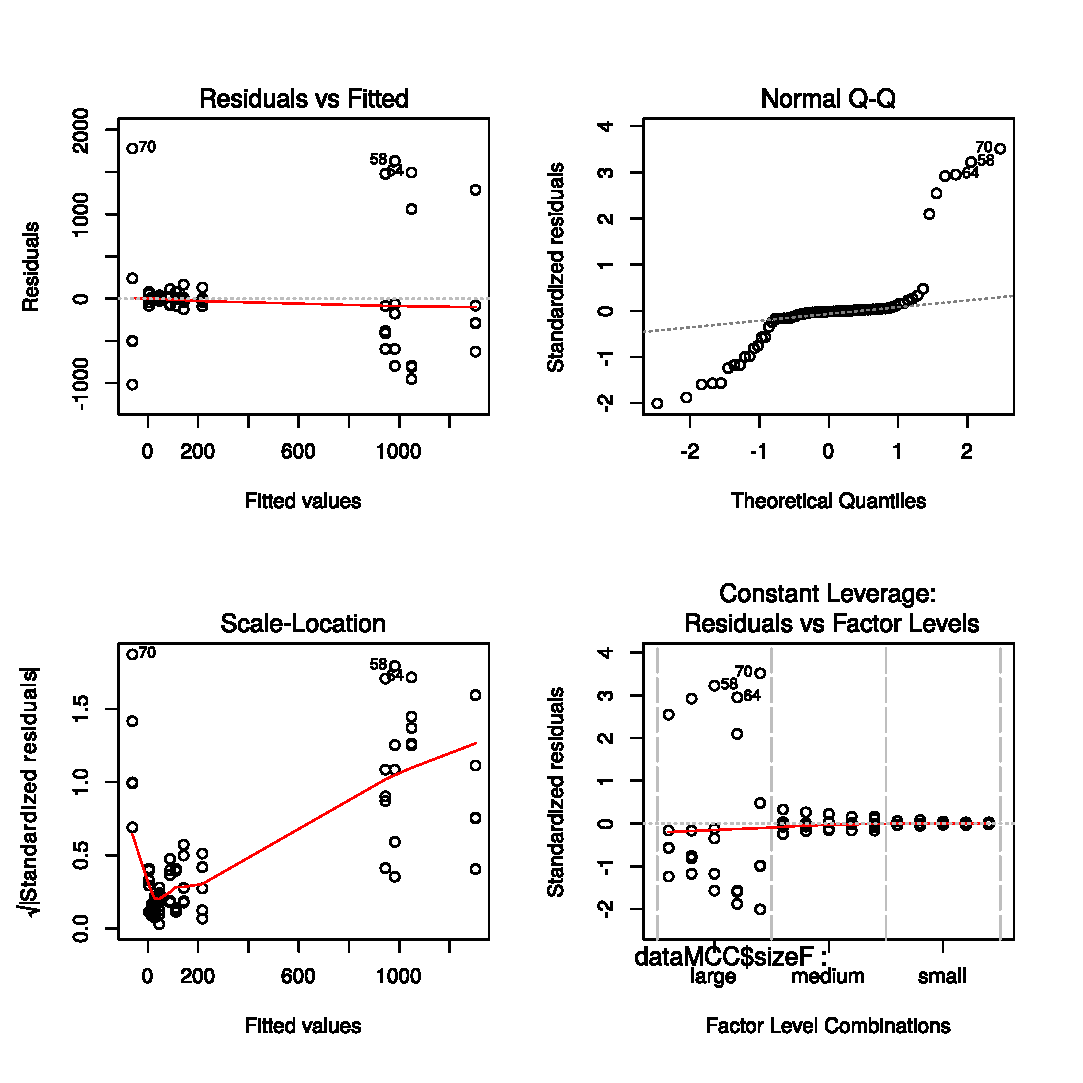
\includegraphics{images/paper/results/ex2_qqplots.eps}
\caption{Delta MCC Experiment Q-Q plots.}\label{fig:ex2_qqplots}
}
\end{figure}

As we can see from the Residuals vs.~Fitted plot, depicted in
Fig.~\ref{fig:ex2_qqplots}, the homogeneity of variance assumption is
not met. To validate this observation we used Levene's Test. In this
test, the null-hypotheses (\(H_0\)) asserts that the variance is equally
distributed. As expected, from our observations of the Residuals vs
Fitted Values plot, the test produced an F-value of 29.856 and a p-value
of 3.61e-10 indicating that we should reject the null hypothesis that
there is a homogeneity of variance.

The Normal Q-Q plot, depicted in Fig.~\ref{fig:ex2_qqplots}, indicates
that the normality of the residuals assumption is also violated. To
validate this observation we conducted both an Anderson-Darling GOF test
against the Normal distribution. In this test the null-hypothesis
(\(H_0\)) is that the empirical distribution is Normal. The results show
the A statistic has a value of 9.9558 and an associated p-value of
\textless{} 2.2e-16 which indicates that we can reject the
null-hypothesis. These results confirm our initial observation that the
results are not normally distributed.

\begin{figure}
\hypertarget{fig:ex2_interaction}{%
\centering
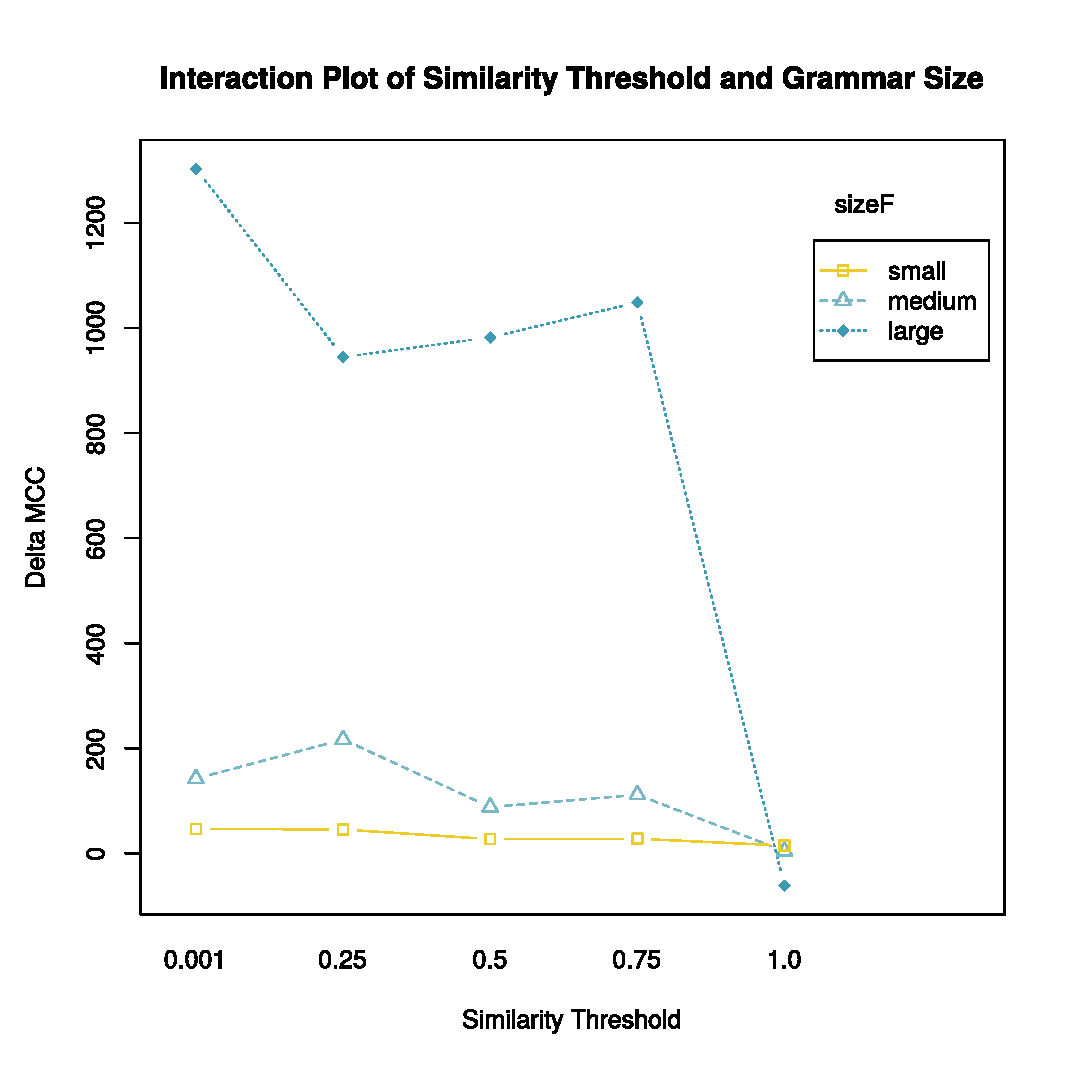
\includegraphics{images/paper/results/ex2_interaction.eps}
\caption{Delta MCC experiment interaction
plot.}\label{fig:ex2_interaction}
}
\end{figure}

The interaction plot, depicted in Fig.~\ref{fig:ex2_interaction},
indicates that there is an interaction between the small and medium
levels as the similarity threshold changes from 0.75 to 1.0. This
indicates that the assumption that the block and treatment do not
interact and that an RCBD design is inappropriate and a factorial design
would be more accurate.

\hypertarget{sec:hyp_tests}{%
\subsection{Hypothesis Testing}\label{sec:hyp_tests}}

This subsection details the results of the \(\Delta HAL\) experiment and
\(\Delta MCC\) experiment. In both cases we initially executed a sample
size analysis to determine the number of replications to execute to
achieve a power level of .95. The results of this analysis indicate the
need to execute a total of 5 replications of each experiment.

\hypertarget{delta-hal-experiment}{%
\subsubsection{\texorpdfstring{\(\Delta HAL\)
Experiment}{\textbackslash Delta HAL Experiment}}\label{delta-hal-experiment}}

We conducted an experiment using a factorial design based on the levels
of the factors size and similarity threshold. Our goal was to determine
if the algorithm when applied had an effect on the change in Halstead
Effort for the combined grammars, as measured by \(\Delta HAL\). Because
of the violations to the assumptions of ANOVA, we opted to utilize
non-parametric methods in our analysis. The initial analysis utilizes a
permutation F-test approach to evaluate if there is any difference among
factor levels. The results was had a p-value of \(<\num{2.2e-16}\)
indicating that we could reject \(H_{1,0}\). We also note that the
interaction indicated in Fig.~\ref{fig:ex1_interaction} was shown to be
significant with a p-value of \(<\num{2.2e-16}\).

We were interested in determining if there was any difference between
the control level (1.0) and other levels of the similarity threshold. To
evaluate this we used Steel's multiple comparison against a control. The
results of this test indicated for each level that there was a
significant difference and that each level the mean \(\Delta HAL\) was
lower than that of the control value.

Finally, we were interested in evaluating the selected levels of the
similarity threshold (excluding control) and if there was an implied
order (that is there is a decreasing order to the change in
\(\Delta HAL\)) as the level value is lowered in the similarity
threshold. To evaluate this we used Jonchkheere's trend test for ordered
differences among classes, which yields a JT statistic value of 767 and
a p-value of \num{4e-4}, when executed using 10000 permutations. This
indicates that we can reject \(H_{3,0}\) that there is no \emph{a
priori} ordering among levels of similarity threshold on median
\(\Delta HAL\).

\hypertarget{delta-mcc-experiment}{%
\subsubsection{\texorpdfstring{\(\Delta MCC\)
Experiment}{\textbackslash Delta MCC Experiment}}\label{delta-mcc-experiment}}

We conducted an experiment using a factorial design based on the levels
of the factors size and similarity threshold. Our goal was to determine
if the algorithm when applied had an effect on the change in Complexity
for the combined grammars, as measured by \(\Delta MCC\). Because of the
violations to the assumptions of ANOVA, we opted to utilize
non-parametric methods in our analysis. The initial analysis utilizes a
permutation F-test approach to evaluate if there is any difference among
factor levels. The results was a p-value of 0.1429 indicating that we
failed to reject \(H_{1,0}\).

We tested if there was any difference between the control level (1.0)
and other levels of the similarity threshold. To evaluate this, we used
Steel's multiple comparison against a control. The results of this test
indicated for each level that there was a significant difference and
that for each level the mean \(\Delta MCC\) was lower than that of the
control value.

Finally, we evaluated the selected levels of the similarity threshold
(excluding control) to if there was a decreasing order to the change in
\(\Delta MCC\) as the similarity threshold values is lowered. To do
this, we used Jonchkheere's trend test for ordered differences among
classes, which yielded a JT statistic value of 742 and a p-value of
\num{1e-04} when executed using 10000 permutations. This indicated that
we can reject \(H_{3,0}\): that there is no \emph{a priori} ordering
among levels of similarity threshold on median \(\Delta MCC\).

\hypertarget{sec:discussion}{%
\section{Interpretation}\label{sec:discussion}}

The results indicate that the proposed merge process embodied in our
algorithm reduces the Halstead Effort and McCabe Cyclomatic Complexity
of a combined grammar at each threshold below the control threshold,
regardless of size. The results also indicate there is a increasing
order to the amount of change in Halstead Effort and cyclomatic
complexity caused by the algorithm as the similarity threshold
decreases. This implies that smaller values of the similarity threshold
produce better results.

Since this was a randomized experiment, one may infer that the
difference in Halstead Effort and McCabe Cyclomatic Complexity was
caused by the difference in similarity threshold. Because the subjects
were selected randomly from the population of ANTLR grammars, we can
extend this inference to that population. But, extending this inference
to the population of grammars as a whole is speculative at best. This
deficiency, however, is minor; the causal relationship is strong even
though it applies only to ANTLR grammars.

\hypertarget{sec:threats}{%
\section{Threats to Validity}\label{sec:threats}}

We focused on threats to the conclusion, construct, internal, and
external validity as detailed by Wohlin et
al.~\cite{wohlinExperimentationSoftwareEngineering2012}. We have
identified no threats to the conclusion and construct validity of this
study, but there is a threat to the internal validity of this study.
Specifically, we selected grammars from the ANTLR repository which
limits the grammars available as well as the formats in which they are
implemented. This is a threat due to the under-representation of the
domain. Additionally, since we restrict our internal representations to
BNF and ANTLR 4 and do not include the ability to utilize TXL, SDF or
other grammar formats, there is a threat to external validity.

\hypertarget{sec:conclusions}{%
\section{Conclusions and Future Work}\label{sec:conclusions}}

In this paper we have developed an algorithmic approach to merging
programming language grammars together. The goal of this approach is to
facilitate the automatic creation of Island Grammars for use in the
development of multi-lingual software analysis tools. We evaluate this
approach through two experiments on combined grammars selected from the
ANTLR grammars-v4 repository. These experiments evaluated the effects of
this approach on changes to Halstead Effort and McCabe Cyclomatic
Complexity of the grammar pairs as they are merged. The results show
that the merging approach reduces the Halstead Effort and Cyclomatic
Complexity when taking both grammar size and similarity threshold into
consideration.

The results of this study are promising and present a potentially
fruitful avenue towards the development of an automated approach to
Island Grammar generation. Island Grammars have been shown to be an
extremely useful approach for the development of multi-lingual analysis
tools, but can be time-consuming to develop.

Immediate avenues for future work are as follows. We intended to conduct
further studies to improve the results herein by expanding the study to
grammars selected from the GrammarZoo \cite{zaytsevGrammarZooCorpus2015}
collection. As part of this we intend to extend the capabilities of this
approach to incorporate TXL and SDF grammars which will also reduce
threats to validity identified in Section~\ref{sec:threats}. The results
herein indicate the promise of this approach and we intend to integrate
it with ongoing work to develop tools which will support the automated
construction of island grammars for use in static analysis and quality
measurement of software systems.

\hypertarget{acknowledgements-1}{%
\section*{Acknowledgements}\label{acknowledgements-1}}
\addcontentsline{toc}{section}{Acknowledgements}

This research is supported by funding from the Ronald E. McNair Post
Baccalaureate Achievement Program at Idaho State University, which is
sponsored by the Department of Education (P217A170169).

\setlength{\parsep}{0pt}

\IEEEtriggeratref{21}
\bibliographystyle{IEEEtran}
\bibliography{references}

\end{document}
